\documentclass[12pt,preprint]{aastex}

\usepackage{subfigure}
\usepackage{wrapfig}

\begin{document}

\title{\huge IRIS Technical Note 34. \\ \vspace{0.4cm}
Numerical Simulations Quicklook Tools}
\date{\hspace{5cm} \large November 14, 2012}

\noindent Prepared by: \\
Juan Mart\'inez-Sykora  \& Viggo H. Hansteen \& Daniel El\'ias N\'obrega Siverio \& Helen Kim \\
Lockheed Martin Solar and Astrophysics Lab. \\
\texttt{juanms@lmsal.com}

\tableofcontents

\section{Summary: Bifrost, simulations \& visualization }

This technical note describes the br\_xmhd package for analyzing and visualizing the 
variables of the 3D radiative MHD simulations computed with Bifrost. In short,
Bifrost code solves the 3D radiative MHD equations including scattering and conduction 
along the magnetic field line \citep{Gudiksen:2011qy}. This code is modular which includes 
other of the most important processes in the chromosphere such as time dependent Hydrogen 
ionization \citet{Leenaarts:2007sf} and partial ionization effects \cite{Martinez-Sykora:2012fk}. 
Typically the domain of these simulations includes from the upper convection zone to the 
lower corona (see ITN 33 for more details and how to download the files). In order to 
analyze the output from these simulations, one can use Crispex (see ITN 35?) or the 
GUI visualization tool br\_xmhd that allows the user to have a quick look at 
3D data interactively. This package can be downloaded from SSW/TBD. 


The simulated data is 4D, i.e., 3D in space and time and the format is saved for each 
variable and each timestep in a different fits file (see ITN 33 for details). SSW/IRIS/Bifrost/?
package allows us to load any variable 
that is pre-saved in a series snapshots of the Bifrost simulations. Predefined variable can
be loaded in any combination possible of a chosen 3D, 2D or 1D format, from the 4D data. 
br\_xmhd tool allows to display the preloaded variable when it has a 3D or 2D 
format. In addition, for Bifrost simulations, SSW/IRIS/Bifrost package allows to 
load (and br\_xmhd display) any derived variables that already is defined in IDL routines 
SSW/IRIS/Bifrost/br\_data\_\_load\_*.pro. br\_xmhd depends on the SSW/IRIS/Bifrost/ package 
and it is recommended to run IDL with Solar Software (SSW) (see section~\ref{sec:dep}).

\section{Setup}

The SSW/IRIS/Bifrost/ IDL library including br\_xmhd.pro can be download from TBD (see 
Section~\ref{sec:dep}). Then, the file must be uncompressed in a chosen path 
(e.g. $\sim$/bifrostcode/IDL/).
	
Please report if you run into troubles doing these steps to TBD (Oslo? Juan? Bart?). 
Next step is setup the .cshrc file in order to have access to this IDL library. 
The .cshrc or equivalent must include: 

\begin{tabular}{l}
setenv BIFROST $<$``location of code''$>$ \\
setenv IDL\_PATH ``+''\$BIFROST``/IDL:+\$IDL\_DIR'' \\
\end{tabular}

Last step before one can start to analyze any of the Bifrost simulations is to download the snapshots
and the necessary files from TBD (see ITN 33). 
The user must download and uncompress (using TBD) these files into the folder where is going to 
launch IDL or SSWIDL.  

\section{Quick Start: A simple example}

Though most of the software should (and does) work with plain IDL, we do suggest 
that you use SSWIDL if you have it available. SSWIDL does not work with bash, so 
stick with (t)csh.

\begin{eqnarray}
&& sswidl \\
&& IDL> br\_select\_fits,fitn \\
&& IDL> d=obj\_new('br\_data',fitn) 
\end{eqnarray}

where fitn is the root name of the fits files of the simulation (ITN33). To continue  

\begin{eqnarray}
&& IDL> d->load,'lgr',43 ~\label{ex:load}\\
&& IDL> r=d->getvar() 
\end{eqnarray}

this put the whole cube of density for timestep 43 into variable $r$. 
Again, the two lines above can be shortened to

\begin{eqnarray}
&& IDL> r=d->getvar('lgr',43) ~\label{ex:load2}
\end{eqnarray}

br\_xmhd can be launch after step~\ref{ex:load} or~\ref{ex:load2} as follows:

\begin{eqnarray}
&& IDL> br\_xmhd,d 
\end{eqnarray}

\clearpage 

\begin{wrapfigure}{r}{0.6\textwidth}
\begin{center}
	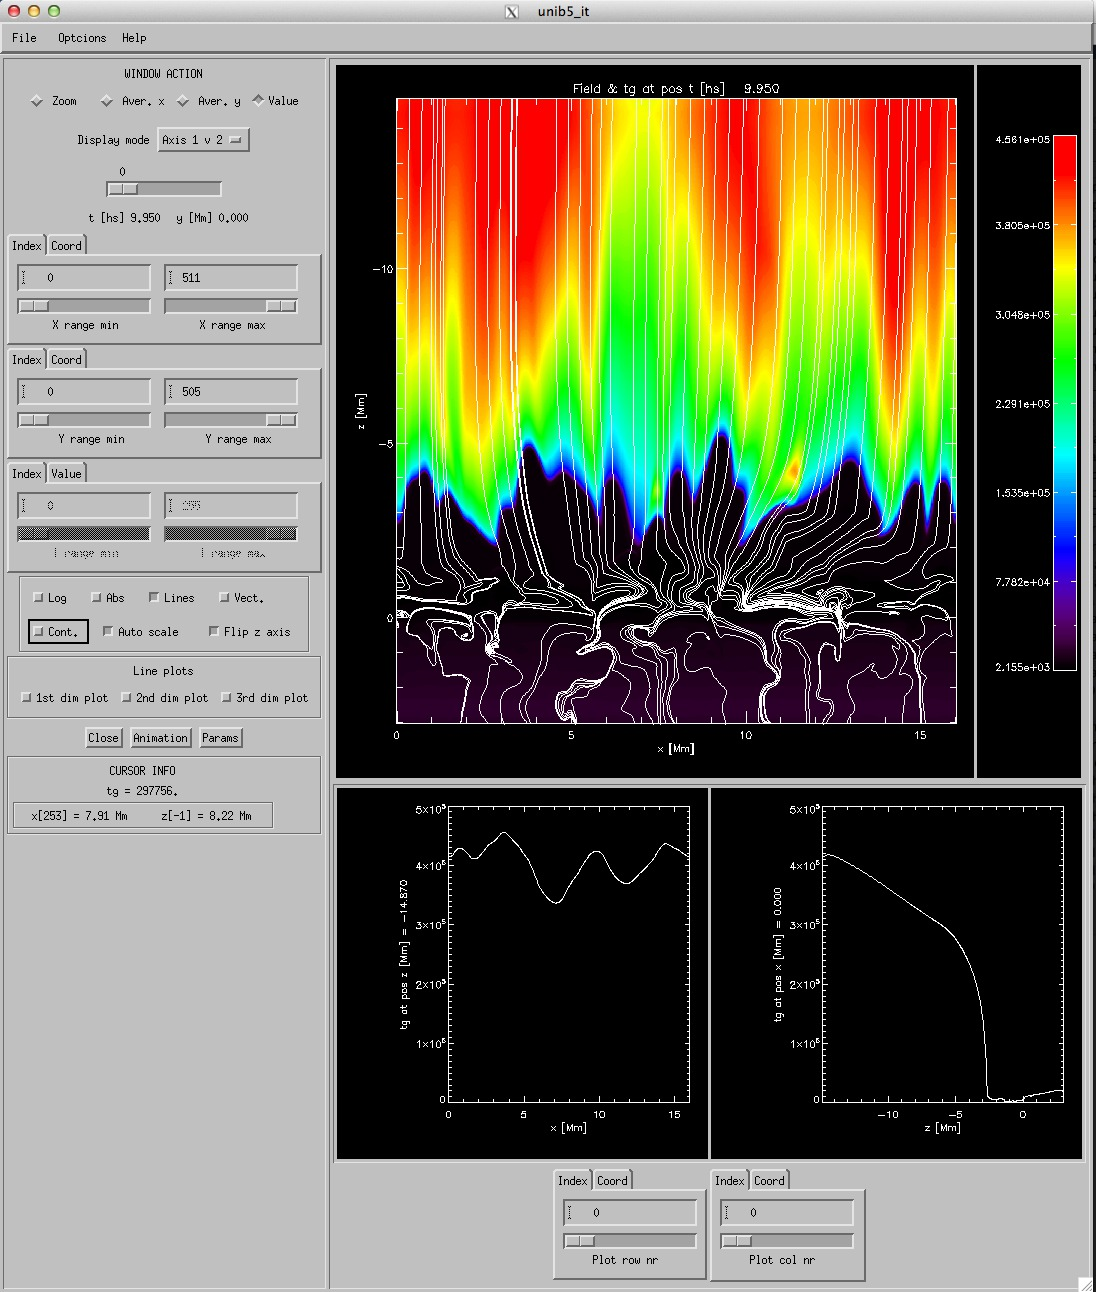
\includegraphics[width=0.6\textwidth]{xmhd.pdf}
\end{center}
\caption{\label{fig:xmhd} Screenshot of the br\_xmhd GUI visualization tool.}
\end{wrapfigure}

where br\_xmhd looks at the variable loaded into object $d$. The user can load any variable 
that is downloaded from the various fits files (see ITN 33), in addition some others that can easily 
be derived from these (e.g., 'px', 'py', 'pz', 'ee'). These derived variables 
are defined in the br\_data\_\_load*.pro routines. Descriptions of the derived variables 
are contained within the comments in these routines. For more information on how to load 
these variables see Section~\ref{sec:oscdata}. All 
these variables will be also printed in the IDL prompt if the variable is an empty space:

 \begin{eqnarray}
&& IDL>d-> load,'\, ',0
\end{eqnarray}

The screenshot of br\_xmhd shown in Figure~\ref{fig:xmhd} displays temperature in a xz 
plane of a 3D Radiative MHD simulation created with the Bifrost code. 
br\_xmhd tool shows a 2D image and let one to raster through the 3rd axis (see Section~\ref{sec:options}).

\section{br\_xmhd options}~\label{sec:options}

The br\_xmhd viewer (see Figure~\ref{fig:xmhd}) is structure as follows:

\begin{itemize}
\item In the top left there is the main plot which is a 2D image in the top-right. 
\item Two 1D plots of a horizontal and a vertical cut of the 2D image. These two plots are located 
below the 2D image.
\item At the left side of the visualization tool there are the various options and rasters that 
lets the user to interact with the visualization. 
\end{itemize}

The options under ``Window action'' allow the user to select a particular rectangular region with the cursor and include: 

\begin{itemize}
\item zooming in,
\item averaging the intensity of the variable in the x direction (along x-axis/columns), 
\item averaging in the y direction (along y-axis/rows). 
\item print out the value in CURSOR INFO. 
\end{itemize}

The display mode changes the ``slice'' of the 2D image.  This only appears when the loaded 
variable is 3D; i.e., 3 spatial dimensions or 2D + time series. There are three possible display modes
(See Figure~\ref{fig:axis}): 

\begin{wrapfigure}{R}{0.5\textwidth}
\vspace{-1.5cm}
\begin{center}
	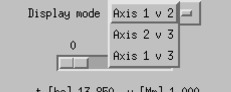
\includegraphics[width=0.48\textwidth]{axis.pdf}
\end{center}
\vspace{-0.56cm}
\caption{\label{fig:axis} Screenshot of the display mode options.}
\vspace{-1.cm}
\end{wrapfigure}

\begin{itemize}
\item 1) Axis 1 v 2 ($x$ vs. $y$, $x$ vs. $z$, or $y$ vs. $z$), 
\item 2) Axis 2 v 3 ($y$ vs. $z$, $y$ vs. $t$, or $z$ vs. $t$), 
\item 3) Axis 1 v 3 ($x$ vs. $z$, $x$ vs. $t$, or $y$ vs. $t$), 
\end{itemize}
which depends on how the variable is loaded. For instance, the example loaded in  
expression~\ref{ex:load} has Axis 1 = $x$, Axis 2 = $y$, and Axis 3 = $z$ (see section~\ref{sec:oscdata}
for details of how to load the data to the object $d$).

%\clearpage 

Other options are:
\begin{itemize}
\item The raster below the display mode allows to move through the 3D data along the axis 
that is not plotted. 
\item Sliding X range min (left) max (right) on top, and Y range min (left) and max (right) at the 
bottom change the image display size and zoom level in the x and y display axis respectively. This 
range can be changed also from the field above the slides. In addition, one can slide or change 
the field using grid points (Index tab) or the values of the axis (Coords tab).  
\item Following similar format as X/Y range min/max, Irange min (left) max (right) changes 
the color contrast. The index ranges from 0 to 255. The Value tab allows to change the limits 
of the colorbar using the units of the variable. Note that this option becomes unavailable when 
Automatic I Scale is chosen. 
\item Logarithm base 10 or absolute value of the variable can be selected.
\item Automatic I Scale button adjusts the image contrast according to the minimum and maximum 
value of the chosen 2D displayed image. 
\item There is also an option to flip the z-axis, which flips the 2D image, so that the image display 
shows the corona on the top of the image and the upper convection zone on the bottom. 
This option only works when the vertical axis of the image is $z$.
\item One can also plot contours, vectors or lines (see Section~\ref{sec:options})
\end{itemize}

Under the main 2D image, there are two line plots. The left line plot graphs 
the value of the variable as a function of the x-axis of the 2D image, while the right 
line plot graphs the value of the variable as a function of the y-axis of the 2D 
image. For example, Figure~\ref{fig:xmhd} displays mode Axis 1 (x-axis in the 
simulation) and Axis 2 (z-axis in the simulation) in the left and right panels respectively. 
The rasters that control the line plots (located at the bottom of the panels) adjust the 
row/column along the perpendicular 
axis in the image. In this case, increasing the ``plot row nr'' raster would increase the $z$ raster 
position. The resulting plot is of the variable as a function of $x$ at that $z$ position. 
Similarly, increasing the ``plot col nr'' raster would increase $x$. 
The resulting plot is of the variable as a function $z$ at that particular $x$ raster position. 
Hence, the rasters move according to a Cartesian grid, with the bottom left corner of the image 
acting as the origin.

In addition to the two 1D plots, br\_xmhd allows to plot any of the three axis of the data. This is selected
in ``Line plots''. When a ``Line plots'' is selected a new window appears where one can 
raster along the other two axis (See Figure~\ref{fig:1dplot}). 

\begin{wrapfigure}{R}{0.5\textwidth}
\vspace{-1.cm}
\begin{center}
	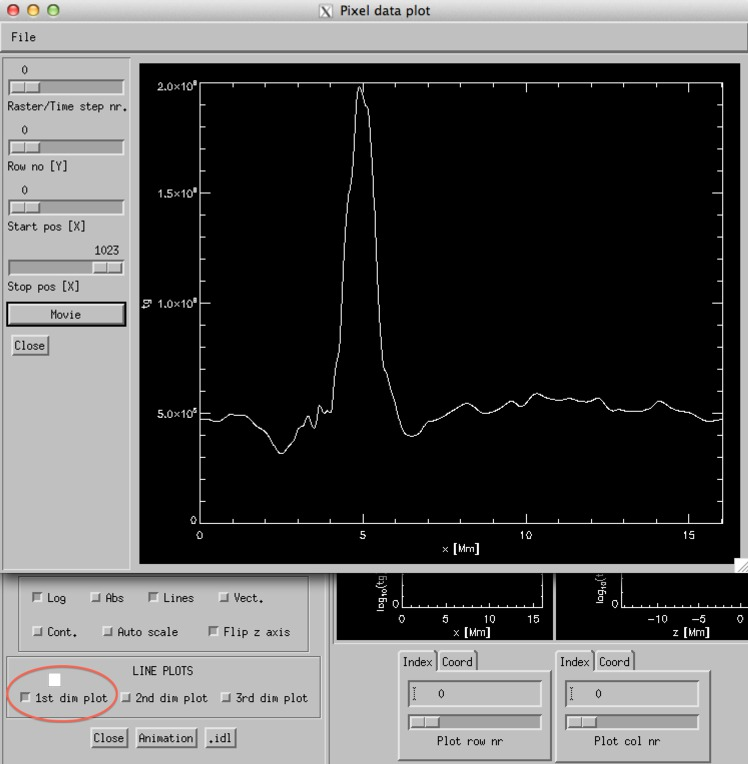
\includegraphics[width=0.48\textwidth]{1dplot.pdf}
\end{center}
\vspace{-0.56cm}
\caption{\label{fig:1dplot} Screenshot of the Lines setup.}
\vspace{-1.cm}
\end{wrapfigure}

The last three bottoms below the LINE PLOTS,  close the br\_xmhd tool (Close button), 
creates an animation of the 2D image (Animation button, see section~\ref{sec:animation}) 
and shows the header of the fits file (params button). 

In the toolbar, going to ``File'' $\rightarrow$ ``Save as'' allows the user to save the image of the variable 
as a .ps or .jpg. One may change the color scheme of the image by going to ``Options'' $\rightarrow$ 
``Colour Table'', which also changes the color bar  (See Figure~\ref{fig:opt}). In addition, one can select 
the limits of the color bar in Setup color bar. One can access to this manual going to 
``Help" $\rightarrow$ ``Manual" or pressing Ctrl+m. Note, most of this options have shortcuts. 

\subsection{Overlying vectors, contours and lines}

In addition to displaying any variable that is saved previously in the Bifrost snapshots or
because it is defined in the SSW/IRIS/Bifrost/ library (br\_data\_load*.pro), br\_xmhd has options 
that calculate and overlay the contours, vectors, or/and lines such as stream lines or magnetic
field liens for a given simulation. These three overlay plots can be setup going to Options 
and selecting the corresponding field, i.e, Line setup, Vector setup and Contour setup. 
The Setup of these over plots can be selected in options as shown in Figure~\ref{fig:opt}

\begin{wrapfigure}{R}{0.5\textwidth}
\vspace{-1cm}
\begin{center}
	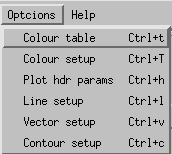
\includegraphics[width=0.48\textwidth]{options.pdf}
\end{center}
\vspace{-0.56cm}
\caption{\label{fig:opt} Screenshot of the Options tab.}
\vspace{-1.cm}
\end{wrapfigure}

Screenshot of main window display when ``Mag field lines'' is selected is shown in 
Figure~\ref{fig:xmhd}. All three setups are quiet intuitive and share several similarities
as detailed below. For example all three setups have in the right side of the window, 
options to select the region where the contours, vectors or lines will be plotted (See 
Figure~\ref{fig:cont},~\ref{fig:vect}, and ~\ref{fig:line} for the vectors and lines setups). 
The top one is for the x axis, and the bottom one is for the vertical axis of the 2D main 
plot. One can choose the range using the Field or the slides. In addition, the range
can be selected using grid axis index or real coordinates (tabs). 

Other similarity in all the three setup options are: 1) one can select the color of the 
lines (Color index field). 2) The last four bottoms draw the overlying plots with the current 
setup without closing the setup window (Draw), save and close the window (Ok), 
return to the Default parameters (Default) and close without saving the current setup. 

\subsubsection{Vector setup}

If one press the button without changing any setup parameter, then the default vector field 
is the velocity. Vector setup options (See Figure~\ref{fig:vect}) allows us to change the 
vector variable to be over plotted, the length, the thickness, the Head size. In addition, 
one can select the number of vectors (along each axis).

\begin{wrapfigure}{R}{0.5\textwidth}
\vspace{-1.cm}
\begin{center}
	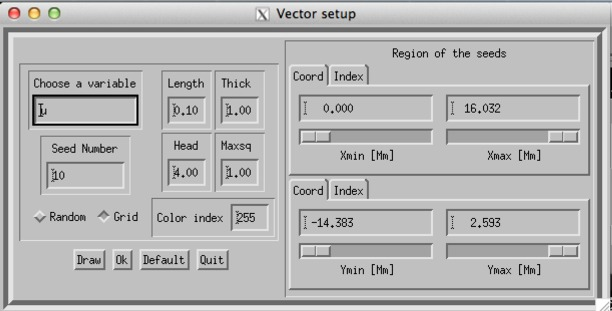
\includegraphics[width=0.48\textwidth]{vectorsetup.pdf}
\end{center}
\vspace{-0.56cm}
\caption{\label{fig:vect} Screenshot of the Vectors setup.}
\vspace{-1.1cm}
\end{wrapfigure}


One can select any vector variable that is saved in the fits files or can be calculated from 
them and are defined in br\_data\_\_load\_*.pro. The first letter of the vector variable must
be filled in the field Choose a variable. Some examples are: for velocity u, for magnetic
field b, for momentum p, for current i or j. 

\subsubsection{Contour setup}

If one press the button without changing any setup parameter, then the default overlying contours 
is plasma beta. Contour setup options allows us to change the variable to be over plotted 
(See Figure~\ref{fig:cont}). Two 
different type of contours can be plotted, one thick line with a selected value in the 
field Thick line value, and several thin lines. The thin lines ranges between the values 
selected in the field Intensity range, and the number of contour thin lines is selected in the 
field Thin lines levels. In addition one can add value labels (selecting the button labels) in 
different plotted contours. 

One can select any variable that is saved in the fits files or can be calculated from 
them and are defined in br\_data\_\_load\_*.pro. The variable name must
be filled in the field Choose a variable. Some examples are: for temperature tg, for
component x of the magnetic field bx, for pressure pg, for energy e. 


\begin{wrapfigure}{R}{0.5\textwidth}
\vspace{-1.cm}
\begin{center}
	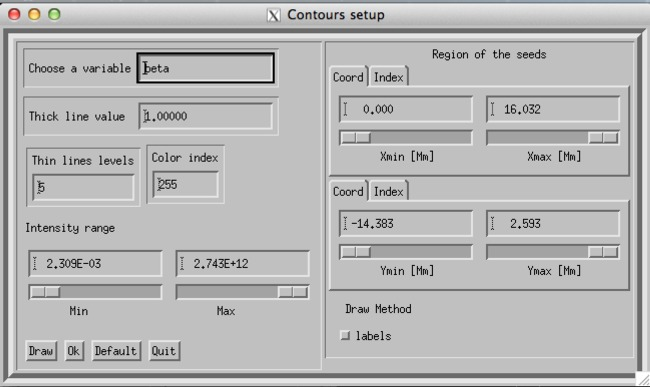
\includegraphics[width=0.48\textwidth]{contours.pdf}
\end{center}
\vspace{-0.56cm}
\caption{\label{fig:cont} Screenshot of the Contours setup.}
\vspace{-1.cm}
\end{wrapfigure}

\subsubsection{Line setup}

Such as shown in Figure~\ref{fig:xmhd}. The field lines are projected in the 2D image where the seed 
points are located in a uniform grid in the chosen 2D plane. 

If one press the Line button without changing any setup parameter, then the default is 
magnetic field lines. Lines setup (See Figure~\ref{fig:line}) allows us to change the variable 
to be over plotted (similar 
way as in the Vector setup). One can select the number of seeds distributed in a uniform grid
within the 2D cut plotted in the main window. 
In addition one can add vectors head (selecting the button Line direction) showing the direction 
of the field lines. 

Drawing the magnetic field lines has an option that allows the user to provide an input field 
lines. For example:
\begin{eqnarray}
&&IDL> d->load,'tg',100\\
&&IDL> br\_bfieldline,'qsmag\_bb01\_it',100,r1,r2,800,800,r0=[[10,6,10],[11,4,5]] \\
&&IDL> br\_xmhd,d,{\rm inputfield}=r1 
\end{eqnarray}

\noindent and ``Lines'' must be selected after launching br\_xmhd. Using this option does not allow
to change the number of seed points, add head vectors or the range of the seeds. 

\begin{wrapfigure}{R}{0.5\textwidth}
\vspace{-1.cm}
\begin{center}
	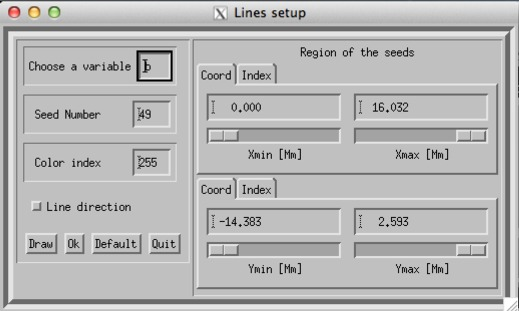
\includegraphics[width=0.48\textwidth]{linesetup.pdf}
\end{center}
\vspace{-0.56cm}
\caption{\label{fig:line} Screenshot of the Lines setup.}
\vspace{-1.cm}
\end{wrapfigure}

\subsection{Animation}~\label{sec:animation}

br\_xmhd has an animation feature that runs through the box along the axis that is not 
displayed in the particular display mode. For example, when only one snapshot is 
loaded and displays $x$ vs. $z$, then the animation will move along $y$-axis. Important, 
this feature woks only when the raster has more than 3 points. 
The animation has basic options at the left side that allow the user to play, pause, rewind, 
and play forward/rewind. The user may also change the frame speed, using ``Animation 
Speed'' and ``Frame increment''. 

Some options from the main window display carry over to the animation feature. These 
options are ``Flip z-axis'',  ``Log (variable)" and ``Abs (variable)''. The default animation 
is in Automatic I scale. However, the animation does not plot the overlying contours, vectors
or lines. 

Similar to the toolbar in the main display window, going to ``File'' $\rightarrow$ ``Save as'' allows the 
user to save the animation as a .ps, .gif (one or all snapshots), .jpg (one or all snapshots), 
or .mpeg file. ``Options'' $\rightarrow$ ``Restrict frame range'' allows the user to choose which frames 
to animate, out of the loaded snapshots. One may change the color scheme by going to 
``Options''  $\rightarrow$ ``Colour Table''.

\subsection{hdr plot}


In $Options->  plot\, hdr\, parameters$ (See Figure~\ref{fig:opt}) one can print 
out if the loaded variable only 
contains a single snapshots or plot the time evolution for any parameter that 
describes the simulation if the loaded variable contains a series of snapshots. 
Once ``Plot hdr params" is selected a new window opens as shown in Figure~\ref{fig:hdr}.


\begin{wrapfigure}{R}{0.5\textwidth}
\vspace{-1.2cm}
\begin{center}
	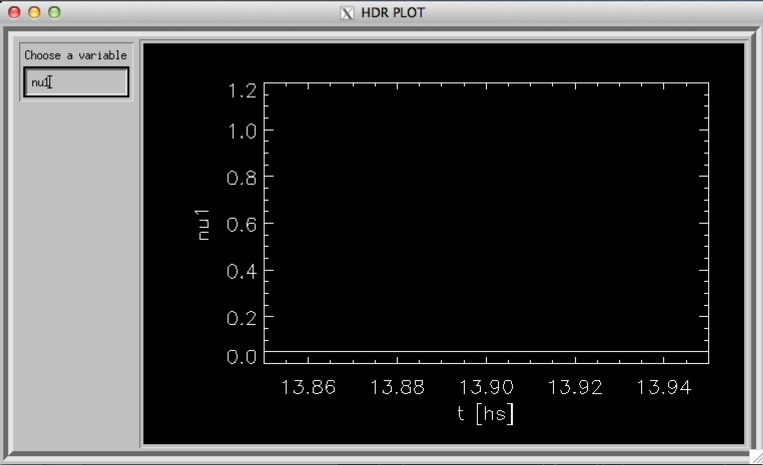
\includegraphics[width=0.48\textwidth]{hdrplot.pdf}
\end{center}
\vspace{-0.56cm}
\caption{\label{fig:hdr} Screenshot of the Plot hdr window.}
\vspace{-1.cm}
\end{wrapfigure}

In the left side one can write inside the ``Choose a variable" the parameter and 
in the right side it will print out the value or plot its time evolution. 

\section{Structure of the software and files (4D data)}

The sofware is built up around three objects: br\_data, br\_hdr, and br\_aux. br\_hdr 
is the superclass of br\_data, while br\_aux is more free standing - though the br\_data 
object contains a pointer to an instance of an br\_aux object. When created (with 
$d=obj\_new('br\_data','<filename>')$) the object 
instance $d$ does not contain any data or header information. This can be loaded with calls to 
various methods as detailed below; but in general the methods will first read the header of the 
file(s) that contain various parameters and the information of the mesh gird, and thereafter the 
fits files that contain the actual data. 

\subsection{The br\_hdr object}

This object has two major roles: to read and store the parameter from the header of the 
fits file. This latter 
task and the data that results is controlled by the br\_aux object as discussed below.

To read a single parameter file (in this case number 800) proceed as follows,

\begin{eqnarray}
&& IDL> d=obj\_new('br\_data','BIFROST\_qs') \\
&& IDL> d->{\rm readparams},800 
\end{eqnarray}

Note that we are using a data 
object to do this read, but since br\_hdr is a superclass of br\_data, one could just as well 
have done the same with a header object: $h=obj\_new('br\_hdr','<snapfileheader>')$ 
thereafter using the same readparams as above. Note also that the readparams method only 
reads a single params file, if you want to read several - for example to plot the effective 
temperature Teff as a function of time - use as follows the readparams method instead:

\begin{eqnarray}
&& IDL> d->{\rm readparams,indgen}(10)+800  \\
&& IDL> print,d->{\rm gett}() \\
&&     79.9994\ \ \ \ \ \ 80.0994\ \ \ \ \ \  80.1994\ \ \ \ \ \  80.3000\ \ \ \ \ \  80.4000 \\
&&      80.5000\ \ \ \ \ \  80.6000\ \ \ \ \ \  80.7000\ \ \ \ \ \ 80.7993 \ \ \ \ \ \  80.8993 \\
&& IDL> print,d->{\rm getteff}() \\
&&       5738.00\ \ \ \ \ \  5736.00\ \ \ \ \ \ 5734.00\ \ \ \ \ \  5747.00\ \ \ \ \ \  5746.00 \\
&&      5746.00\ \ \ \ \ \   5745.00\ \ \ \ \ \  5745.00\ \ \ \ \ \  5725.00\ \ \ \ \ \  5724.00 \\
&& IDL> plot,d->{\rm gett}(),d->{\rm getteff}(),/yn
\end{eqnarray}

\noindent etc. The readparams method is defined in the data object, not the br\_hdr object, 
so you will need to use an instance of a br\_data object to call it.

There are a number of methods available to access 
the various grid variables:

\begin{tabular}{l}
function br\_hdr::getmx \\
function br\_hdr::getxm \\
function br\_hdr::getx \\
function br\_hdr::getxmdn \\
function br\_hdr::getdxidxup \\
function br\_hdr::getdxidxdn \\
function br\_hdr::getdx1d \\
function br\_hdr::getdx 
\end{tabular}

\noindent and equivalent for the $y$ and $z$ grids. Thus, for example, print, $d->getz()$ prints the $z$ grid.

As should be obvious, the variables contained in the params file can be accessed with 
$get<var\_name>$ methods.

It is often not necessary to access the readparams and readmesh methods directly, these are 
automatically invoked when reading data using the load or getvar methods of the 
br\_data object described below. 

\subsection{The br\_data object}\label{sec:oscdata}

The central method(s) of the br\_data object are load and getvar; the most important keywords are 
shown here

\begin{tabular}{l}
pro br\_data::load,varname,isnap,ix=ix,iy=iy,iz=iz,bdrchk=bdrchk,log=log \\
function br\_data::getvar,win,isnap,ix=ix,iy=iy,iz=iz,bdrchk=bdrchk,log=log
\end{tabular}

The only difference between these is that the getvar returns a copy of the data cube requested. 
Both methods read a certain 3D section of the 4D data cube depending on the values given for the 
$ix$, $iy$, $iz$ slices. E.g. setting $iy=0$ (the default) will result in reading in the variable varname from the 
snapshots given by the isnap array for the $iy=0$ slice of the cube. If a scalar isnap is given the entire 
3D spatial cube is read in. Examples of loading ten snapshots in the $xy$ plane at the z-axis grid 
position $iz=10$ are as follows:

\begin{eqnarray}
&& IDL> d->load,'tg',800+indgen(10),iz=10 \\
&& IDL> tg=d->getvar('tg',800+indgen(10),iz=10) \\
\end{eqnarray}

In the former case the variable contained in the object can be accessed a-posterior with a 
blank getvar call

\begin{eqnarray}
&& IDL> tg=d->getvar()
\end{eqnarray}

The variables allowed to be read in saved in the various fits files, e.g.,  
(`lgr', `ux', `uy', `uz', `lge', `bx', `by', `bz','lgtg','lgne','lgpg') 
and a number of derived variables such as the speed of sound (`cs'), the momentum 
(`px',`py',`pz'), etc (see the br\_data\_\_load*.pro routines and Section~\ref{sec:dep}). 
The name assigned to the most common variables is listed in Table~\ref{tab:var}.

Once the requested variable is loaded, it can be viewed with standard plotting 
routines or with the br\_xmhd viewer (see above), designed to show the 3D cube loaded 
into a br\_data object $d$:

\begin{eqnarray}
IDL> br\_xmhd,d
\end{eqnarray}

There are also a limited 
number of methods for returning reduced data such as the horizontal average ($d->hav()$), 
the maximum ($d->hmax()$) or the minimum ($d->hmin()$). 

\subsection{The br\_aux object}

The br\_aux object was mainly designed to keep data relevant for plotting (axis names, window numbers, 
etc) and displaying the data cubes, for finding auxiliary data, but there are a number of methods 
that might be of interest to the ``general'' user. Note that there is an br\_aux object associated 
with the br\_data object that can be accessed using the 
$d->getaux()$ method, and some methods are also directly callable via the br\_data object such as

\begin{eqnarray}
&& idl> aux=obj\_new('br\_aux') \nonumber\\
&& idl> print,aux->getabund('he2\_303\_p')\nonumber\\
&& idl> print,aux->getwvl('he2\_303\_p')\nonumber\\
&& idl> print,aux->awgt('he2\_303\_p')   \nonumber
\end{eqnarray}

Note, not all the function in aux are available without the equation of state table.

\section{Dependences}~\label{sec:dep}

Table~\ref{tab:routines} lists the routines that directly or indirectly are required in order to 
use br\_xmhd.pro with its full performance. The table indicates the folder of the 
routine, the name, br\_xmhd.pro dependence on the routine, and a short description 
of the routine. The dependence is score as follows:

\begin{itemize}
\item indirectly = BR\_XMHD does not use the routine and nor the routines used in 
BR\_XMHD.pro. However, it facilitates to do some things.
\item semi-directly = BR\_XMHD does not use the routine, and the routines used in 
BR\_XMHD.pro are dependent on it. 
\item directly = BR\_XMHD.pro uses the routine.
\item low = one can run BR\_XMHD without problems. These routines are useful to load any other 
variable that are not saved in the snap and aux files. 
\item medium = one can run BR\_XMHD without problems without the routine. 
However, there will be variables that can not be read.
\item medium-high = one can run BR\_XMHD but some features can not be used such as drawing 
field lines.
\item high = one can not use BR\_XMHD without them. 
\end{itemize}

\begin{table}[h!]
\caption{list of IDL routines related with br\_xmhd.pro \label{tab:routines}}
\begin{tabular}{ p{1.4cm}|p{4.5cm}|  p{3.3cm}  | p{6cm} l}
Path & name & type of dependence & description \\
\hline               
 objects &  br\_getsnapind & indirectly, low & gets indices of snap files for given root file name \\
 \hline
   &  br\_getntime & directly, high & gets number of time steps \\
 \hline
   & br\_select\_fits  & indirectly, low & selects one fits file from directory  \\
 \hline
   & br\_aux\_\_define  & semi-directly, high & is the main program of the br\_aux object \\	
 \hline
   & br\_data\_\_define  & directly, high &  is the main program of the br\_data object  \\
 \hline
   & br\_hdr\_\_define & directly, high & is the main program of the br\_hdr object.  \\
 \hline
   & br\_hion\_\_define  & demi-directly, high &  is the main program of the br\_hion object, i.e., 
   				object related to time dependent H ionization \\
 \hline
   & br\_data\_\_load\_fitsbvar & directly (beta), medium-high & defines new variables that are 
   				dependent on the magnetic field, e.g., plasma beta, Alfv\'en velocity,   \\
 \hline
   & br\_data\_\_load\_fitsothers & semi-directly, medium & defines ``other'' variables, emissivity 
   				of EUV lines using CHIANTI and non logarithmic variables.  \\
 \hline
   & br\_data\_\_load\_fitspart & semi-directly, medium  & defines new variables that are 
   				as a function of particle, e.g., current per particle.  \\
 \hline
   & br\_data\_\_load\_fitspoynting  & semi-directly, medium & defines the Poynting flux.  \\
 \hline
   & br\_data\_\_load\_fitsvaror  & semi-directly, medium & defines new variables that are 
   				divided per density, e.g. the momentum ($p_{x}=u_{x} \rho$). \\
 \hline
   & br\_data\_\_load\_fitsvectoper  & semi-directly, medium & calculates operations between 
   				variables such as gradients, vectorial products etc. \\
\hline               
fits   & br\_make\_\_fits\_level3  & None & calculates level 3 data. \\
\end{tabular}
\end{table}

\clearpage			

\begin{table}[h!]
\caption{list of IDL routines related with br\_xmhd.pro \label{tab:routines}}
\begin{tabular}{ p{1.4cm}|p{4.5cm}|  p{3.3cm}  | p{6cm} l}
Path & name & type of dependence & description \\
\hline
analysis   & br\_iion  & semi-directly, medium  & calculates the emissivity for EUV lines using the
   				$G(T,n_{e})$ tables. \\
   \hline
   & br\_bline & directly (magnetic field lines), medium-high & calculates field line for a 
				 specific seed point \\
   \hline
   & br\_bfieldline & directly (magnetic field lines), medium-high & calculates field line 
   				(using b\_line.pro) for  several seed points.
 \\   \hline
   & br\_chianti\_ build\_goftne\_nsens  & semi-directly, medium & creates $G(T,n_{e})$ (uses SSW/CHIANTI) 
		   		tables of synthetic EUV lines using optically thin approx. \\
\hline               
ql   & br\_locval & semi-directly & finds the grid position of a particular spatial position (uses where).  \\
\hline
   & br\_plot\_image.pro & directly, high (2D image) & plots the 2D image.  \\
   \hline
   & br\_stretch & directly, high & stretch the vertical axis to an uniform grid  \\
   \hline
   & br\_xmhd & It is the main program & It is the main br\_xmhd program  \\
\end{tabular}				
\end{table}

\begin{table}[h!]
\caption{List of most variables names that can be read in IDL \label{tab:var}. Note, in order to read  
these variables must be saved in the .snap file, .aux file or derived in the br\_data\_\_load*.pro 
routines. This is not the a complete list.}
\begin{tabular}{p{0.8cm} |p{3.3cm} || p{4.5cm} | p{5.7cm} }
\hline
'r' & mass density & 'px', 'py', 'pz' & Momentum  \\
\hline
'e' & energy & 'ne8\_343\_p', (initials + ionization level + wavelength in \AA) & EUV emission \\ 
\hline
'ee' & internal energy & 'ux', 'uy', 'uz' & Velocity \\
\hline
'pg' & gas pressure & '?2', e.g. $B^2$= 'b2'  & Square of a vector \\
\hline
'tg' & temperature & 'bx', 'by', 'bz' & Magnetic field \\
\hline
'lgr' & $\log(r)$  & 'lgtg' & $\log(tg)$\\
\hline
'ne' & electron density  &  mod?,e.g., $modu=|u|$ & Vector module \\
\hline
'pb' & magnetic pressure & 'lgpg' & $\log (pg)$  \\
\hline
pt' & total pressure  & 'beta' & Plasma beta  \\
\hline
's' & entropy & 'lgne' & $\log(ne)$  \\
\hline
'cs' & sound speed & ?perp?', '?par?', & ? (e.g., b) perpendicular to ? (e.g., u), ? (e.g., e) parallel to ? \\
\hline
'va' & Alfven speed 
 \end{tabular}
\end{table}

\bibliographystyle{aa}
\bibliography{aamnemonic,collectionbib}

\end{document}
